\iffalse
\chapter{2022}
\section{xe}
\author{EE24BTECH11030}
\fi
    \item Which of the following statement(s) is/are true for streamlines in a steady incompressible flow?
    \begin{enumerate}
        \item Two streamlines cannot intersect each other.
        \item Flow rate increases between two diverging streamlines.
        \item Flow rate decreases between two diverging streamlines.
        \item Stream function has a constant value along a streamline.
    \end{enumerate}

    \bigskip

    \item A flow has a velocity potential given by $\Phi = Ax^3$ where $A$ is a non-zero constant. Which of the following statement(s) is/are true about the flow?
    \begin{enumerate}
        \item The flow is incompressible.
        \item The flow is irrotational.
        \item The flow has local acceleration.
        \item The flow has convective acceleration.
    \end{enumerate}

    \bigskip

    \item A boundary layer develops due to a two-dimensional steady flow over a horizontal flat plate. Consider a vertical line away from the leading edge which extends from the wall to the edge of the boundary layer. Which of the following quantity/quantities is/are not constant along the vertical line? $u$ and $v$ represent the components of velocity in the direction along the plate and normal to it, respectively, and $x$ is taken along the length of the plate while $p$ is the pressure. Neglect body forces.
    \begin{enumerate}
        \item $u$
        \item $\frac{\partial u}{\partial x}$
        \item $v$
        \item $p$
    \end{enumerate}
\bigskip
    \item A 10 kg mass placed on an infinitely long horizontal massless flat platform is to be supported by a steady vertical water jet as shown in the figure. The diameter of the jet is 5 cm. What minimum average velocity is required to hold the mass in place?
\begin{figure}[H] % Use [H] to force the figure to appear exactly where it is placed
\centering
\scalebox{0.8}{ % Adjust the scaling factor as needed
\begin{circuitikz}
\tikzstyle{every node}=[font=\LARGE]

% Positive sign
\node[font=\normalsize] at (-2.75,1.75) {+};

% Horizontal lines
\draw (1,1.75) -- (8.25,1.75);
\draw (1,1.5) -- (8.25,1.5);
\draw (1,0.75) -- (4.25,0.75);
\draw (5.25,0.75) -- (8.25,0.75);

% Vertical and horizontal lines for small rectangle
\draw (4.25,0.75) -- (4.25,-1.5);
\draw (5.25,0.75) -- (5.25,-1.5);
\draw (4.25,-1.5) -- (5.25,-1.5);

% Diagonal lines for trapezoid
\draw (3.25,2.75) -- (4,3.5);
\draw (4,3.5) -- (5.5,3.5);
\draw (3.25,2.75) -- (3.25,1.75);
\draw (5.5,3.5) -- (6.25,2.75);
\draw (6.25,2.75) -- (6.25,1.75);

% Circle at top center
\draw (4.75,3.75) circle (0.25cm);

% Horizontal line at the bottom of rectangle
\draw (4.25,-0.25) -- (5.25,-0.25);

% Mass label
\node[font=\LARGE] at (4.75,2.5) {10 Kg};

% Double arrow for 5cm label
\draw [<->, >=Stealth] (4.25,-0.75) -- (5.25,-0.75);
\node[font=\normalsize] at (4.75,-1) {5cm};

\end{circuitikz}
}
\end{figure}
    
    Assume $\rho_{\text{water}} = 1000$ kg/m$^3$, $g = 10$ m/s$^2$ and $\pi = 3.14$. Neglect friction.
    \underline{\hspace{1cm}} (Round off to two decimal places.)
    \bigskip

    \item Consider an inviscid flow through a smooth pipe which has a pitot-static tube arrangement as shown. Find the centre-line velocity in the pipe.

    Consider that the density of the fluid is 1000 kg/m$^3$, acceleration due to gravity is 10 m/s$^2$, and the specific gravity of the manometric fluid is 11.
    \begin{figure}[!ht]
\centering
\begin{circuitikz}[scale=1] % Adjust scale as needed
\tikzstyle{every node}=[font=\normalsize]
\begin{scope}[scale=1] % You can change the scale factor here
    \draw [short] (5.75,10.75) -- (5.75,5.5);
    \draw [short] (7,10.75) -- (7,5.5);
    \draw [short] (5.75,10.75) .. controls (6.25,11.25) and (6.75,11) .. (7,10.75);
    \draw [short] (5.75,10.75) .. controls (6.25,10.25) and (6.75,10.5) .. (7,10.75);
    \draw [short] (5.75,5.5) .. controls (6.25,5) and (6.5,5) .. (7,5.5);
    \draw [short] (5.75,5.5) .. controls (6.25,6) and (6.75,5.75) .. (7,5.5);
    \draw [->, >=Stealth] (6.25,12) -- (6.25,10);
    \draw [dashed] (4,10) -- (5,10);
    \draw [dashed] (4.25,6) -- (5,6);
    \draw [dashed] (4.25,6) -- (4,6);
    \draw [<->, >=Stealth] (4.5,10) -- (4.5,6)node[pos=0.5, fill=white]{300mm};
    \draw [short] (7,9.75) -- (9.5,9.75);
    \draw [short] (7,9.5) -- (9.25,9.5);
    \draw [short] (9.25,9.5) -- (9.25,6.5);
    \draw [short] (9.5,9.75) -- (9.5,6.5);
    \draw [short] (6.5,6.75) -- (6.5,6.5);
    \draw [short] (6.5,6.5) -- (7.75,6.5);
    \draw [short] (7.75,6.5) -- (7.75,5.75);
    \draw [short] (7.75,5.75) -- (9.25,5.75);
    \draw [short] (9.25,5.75) -- (9.25,6.75);
    \draw [short] (6.25,6.75) -- (6.25,6.5);
    \draw [short] (6.25,6.5) -- (6.25,6.25);
    \draw [short] (6.25,6.25) -- (7.5,6.25);
    \draw [short] (7.5,6.25) -- (7.5,5.5);
    \draw [short] (7.5,5.5) -- (9.5,5.5);
    \draw [short] (9.5,5.5) -- (9.5,6.5);
    \draw [dashed] (9.25,6.5) -- (10.25,6.5);
    \draw [dashed] (7.5,5.75) -- (10.25,5.75);
    \draw [<->, >=Stealth] (10,6.5) -- (10,5.75)node[pos=0.5,right, fill=white]{20 mm};
    \draw [dashed] (7.5,5.5) -- (8,5.75);
    \draw [dashed] (7.75,5.5) -- (8.25,5.75);
    \draw [dashed] (8,5.5) -- (8.5,5.75);
    \draw [dashed] (8.25,5.5) -- (8.75,5.75);
    \draw [dashed] (8.5,5.5) -- (9,5.75);
    \draw [dashed] (8.75,5.5) -- (9.25,5.75);
    \draw [dashed] (9,5.5) -- (9.5,5.75);
    \draw [dashed] (9.25,5.5) -- (9.5,5.75);
    \draw [dashed] (9.25,5.75) -- (9.5,6);
    \draw [dashed] (9.25,6) -- (9.5,6);
    \draw [dashed] (9.25,6) -- (9.5,6.25);
    \draw [dashed] (9.25,6.25) -- (9.5,6.5);
    \node [font=\normalsize] at (5,12) {Direction};
    \node [font=\normalsize] at (4.5,11.5) {of};
    \node [font=\normalsize] at (5.25,11.5) {flow};
\end{scope}
\end{circuitikz}
\end{figure}

    \begin{enumerate}
        \item 2 m/s
        \item 3 m/s
        \item 5 m/s
        \item 7 m/s
    \end{enumerate}
\bigskip
    \item The speed of propagation, $c$, of a capillary wave depends on the density of the fluid, $\rho$, the wavelength of the wave, $\lambda$, and the surface tension, $\sigma$. If the density and wavelength remain constant, halving the surface tension would lead to a new velocity, $c'$, given by
    \begin{enumerate}
        \item $c' = \sqrt{2}c$
        \item $c' = \frac{c}{\sqrt{2}}$
        \item $c' = \frac{c}{2}$
        \item $c' = 2c$
    \end{enumerate}
    
    \item A two-dimensional flow field is described by a combination of a source of strength $m$ at the origin and a uniform flow, $U$, in the positive $x$-direction such that the velocity potential is given by
    \[
    \phi = Ux + \frac{m}{2\pi} \ln \sqrt{x^2 + y^2}
    \]
    The stagnation streamline is shown in the figure. Find the distance $a'$.
    \begin{enumerate}
        \item $\frac{m}{U}$
        \item $\frac{2m}{U}$
        \item $\frac{8m}{U}$
        \item $\frac{m}{2U}$
    \end{enumerate}

    \item A typical boundary layer over a flat plate has a linear velocity profile with zero velocity at the wall and freestream velocity, $U_\infty$, at the outer edge of the boundary layer. What is the ratio of the momentum thickness to the thickness of the boundary layer?
    \begin{enumerate}
        \item $\frac{1}{2}$
        \item $\frac{1}{4}$
        \item $\frac{1}{6}$
        \item $\frac{1}{3}$
    \end{enumerate}
    
    \item Identify the configuration(s) in which steady two-dimensional internal flow may show boundary layer separation if the flow direction is left to right.
    \begin{enumerate}
        \item
\begin{tikzpicture}
    % Shaded area above the first line
    \fill[pattern=north east lines, pattern color=gray] (-1, 2.6) rectangle (5, 3);
    \draw[ultra thick, black, line cap=round, line width=1pt] (-1, 2.6) -- (5, 2.6);

    % Shaded area below the second line
    \fill[pattern=north east lines, pattern color=gray, rotate around={15:(2.5,0.3)}] (-1,0) rectangle (6, -0.4);
    \draw[ultra thick, black, line cap=round, line width=1pt, rotate around={15:(2.5,0.3)}] (-1, 0) -- (6, 0);
\end{tikzpicture}
        \item \begin{tikzpicture}
    % Shaded area above the first line
    \fill[pattern=north east lines, pattern color=gray] (-1, 2.6) rectangle (5, 3);
    \draw[ultra thick, black, line cap=round, line width=1pt] (-1, 2.6) -- (5, 2.6);

    % Shaded area below the second line
    \fill[pattern=north east lines, pattern color=gray,] (-0.8,1.5) rectangle (5, 1.1);
    \draw[ultra thick, black, line cap=round, line width=1pt,] (-0.8,1.5) -- (5,1.5);
\end{tikzpicture}
        \item
\begin{tikzpicture}
    % Shaded area above the first line
    \fill[pattern=north east lines, pattern color=gray] (-1, 2.6) rectangle (5,3);
    \draw[ultra thick, black, line cap=round, line width=1pt] (-1, 2.6) -- (5, 2.6);

     % Shaded area below the second line
    \fill[pattern=north east lines, pattern color=gray, rotate around={-15:(2.5,0.3)}] (-1,0) rectangle (5.3, -0.3);
    \draw[ultra thick, black, line cap=round, line width=1pt, rotate around={-15:(2.5,0.3)}] (-1, 0) -- (5.2, 0);
\end{tikzpicture}
        \item 
\begin{tikzpicture}
    % Horizontal line with shadow above
    \fill[pattern=north east lines, pattern color=gray] (-1.2, 2.65) rectangle (5.2, 2.85);
    \draw[ultra thick, black, line cap=round, line width=1pt] (-1, 2.6) -- (5, 2.6);

    % L-shaped line with shadow below
   \fill[pattern=north east lines, pattern color=gray] (-1.2, 1.05) -- (2.1, 1.05) -- (2.1, -0.3) -- (5.3, -0.3) -- (5.3, -0.5) -- (1.8, -0.5) -- (1.8, 0.8) -- (-1.2, 0.8) -- cycle;
    \draw[ultra thick, black, line cap=round, line width=1pt] (-1.2, 1) -- (2.1,1) -- (2.1, -0.3) -- (5.3,-0.3);
\end{tikzpicture}
    \end{enumerate}

\item Consider steady fully developed flow of a liquid through two large horizontal flat parallel plates separated by a distance of $2$ mm. One of the plates is fixed and the other plate moves at a speed of $0.5$ m/s. What is the magnitude of the pressure gradient (in Pa/m) in the direction of the flow required to ensure that the net flow through the plates is zero?

Dynamic viscosity of the liquid is $5 \times 10^{-4}$ Ns/m$^2$

(Round off to the nearest integer)
\bigskip

\item Consider two-dimensional turbulent flow of air over a horizontal flat plate of length $1$ m. Skin friction coefficient at a length $x$ from the leading edge of the plate is obtained as:
\[
c_f = \frac{0.06}{\left( Re_x \right)^{0.2}}
\]
where, $Re_x$ is the local Reynolds number.

Find out the drag force per unit width (in N/m$^2$) on the plate if the free stream air velocity is $10$ m/s.

Density and dynamic viscosity of air are given as $1.2$ kg/m$^3$ and $1.83 \times 10^{-5}$ Ns/m$^2$, respectively.

(Round off to three decimal places)
\begin{figure}[h!]
    \centering
    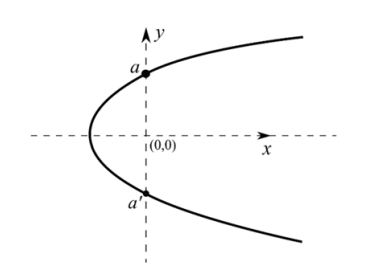
\includegraphics[width=\textwidth]{GATE-yearwise/GATE(11)/figs/fig1.png}
    \caption{}
    \label{fig:fig1}
\end{figure}
\newpage

\item For an inviscid fluid with density $1$ kg/m$^3$, the Cartesian velocity field is given as:
\[
\mathbf{u} = (-2x + y)i + (2x + y)j \, \text{m/s}
\]
Neglecting the body forces, find the magnitude of pressure gradient in (Pa/m) at $(x, y) = (1 \text{ m}, 1 \text{ m})$ at $t = 1$ s.

(Round off to two decimal places)
\bigskip

\item Consider a lawn sprinkler with horizontal arms of radius, $a = 10$ cm which has water inlets vertically through the centre, as shown in the figure. The exit area of the jet is $25$ cm$^2$ and the jet velocity is $1$ m/s. The water is ejected orthogonal to the sprinkler arm and the jet makes an angle of $60^\circ$ with the horizontal plane. Find the torque (in N$\cdot$m) required to hold the sprinkler stationary.

Consider water density $1000$ kg/m$^3$. Neglect the effects of friction and gravity.

(Round off to two decimal places)
\begin{figure}[!ht]
    \centering
    % First diagram
    \begin{minipage}{0.45\textwidth} % Set width for the first diagram
        \centering
        \begin{circuitikz}[scale=1]
            \tikzstyle{every node}=[font=\normalsize]
            \begin{scope}[line cap=round] % Rounded ends for smoother connections
                % Main horizontal pipes
                \draw [short] (5,7.75) -- (12.5,7.75);
                \draw [short] (4.75,7.25) -- (8.25,7.25);

                % Vertical pipes and connections
                \draw [short] (8.25,7.25) -- (8.25,5.25);
                \draw [short] (9.25,7.25) -- (9.25,5.5);
                \draw [short] (9.25,7.25) -- (13.25,7.25);
                \draw [short] (13.25,7.25) -- (13.25,8.25);
                \draw [short] (12.5,7.75) -- (12.5,8.25);
                \draw [short] (4.75,7.25) -- (4.5,7.25);
                \draw [short] (5,7.75) -- (5,8.25);
                \draw [short] (4.5,7.25) -- (4.25,7.25);
                \draw [short] (4.25,7.25) -- (4.25,8.25);
                \draw [short] (8.25,5.25) -- (9.25,5.25);
                \draw [short] (9.25,5.25) -- (9.25,5.75);

                % Front oval (left side) filled and aligned with pipe end
                \fill[white] (4.75,8.25) ellipse (0.5cm and 0.25cm);
                \draw (4.75,8.25) ellipse (0.5cm and 0.25cm);
                \draw [short] (4.25,8.25) .. controls (4.5,8.5) and (5,8.5) .. (5,8.25);

                % Back oval (right side) filled and aligned with pipe end
                \fill[white] (12.75,8.25) ellipse (0.5cm and 0.25cm);
                \draw[dashed] (12.75,8.25) ellipse (0.5cm and 0.25cm);
                \draw [short] (12.5,8.25) .. controls (12.75,8.5) and (13.25,8.5) .. (13.25,8.25);

                % Dimension and direction indicators
                \draw [<->, >=Stealth] (4.75,7) -- (8,7) node[pos=0.5, fill=white]{a};
                \draw [->, >=Stealth] (4.5,8.25) -- (4.5,9.5);

                % Labels
                \node [font=\large] at (8.5,4.75) {Front view};
                \node [font=\normalsize] at (4.5,10) {V};
            \end{scope}
        \end{circuitikz}
    \end{minipage}%
    \hspace{0.15\textwidth} % Increased horizontal space between diagrams
    % Second diagram
    \begin{minipage}{0.8\textwidth} % Increase minipage width to make the diagram larger
    \centering
    \resizebox{0.9\textwidth}{!}{% Scale to 90% of the text width
        \begin{circuitikz}
            \tikzstyle{every node}=[font=\normalsize]
            \draw [short] (6.25,8.25) -- (6.25,5);
            \draw [short] (6.25,5) -- (7.25,5);
            \draw [short] (7.25,5) -- (7.25,8);
            \draw [short] (7.25,8) -- (7.25,8.25);
            \draw [short] (6.25,8.25) -- (5.75,9);
            \draw [short] (6.25,8.25) -- (7,9.25);
            \draw [short] (7.25,8.25) -- (7.75,9);
            \draw [dashed] (5.75,8.25) -- (8.25,8.25);
            \draw [->, >=Stealth, dashed] (6.75,8.25) -- (8,10);
            \draw [short] (6.75,8.75) -- (6.25,9.25);
            \draw [short] (5.75,9) .. controls (5.5,9.5) and (6,9.5) .. (6.25,9.25);
            \draw [short] (15.25,12.5) -- (15,12.5);
            \draw [short] (7,9.25) .. controls (7.5,9.5) and (7.75,9.5) .. (7.75,9);
            \draw [short] (7,9.25) .. controls (7.25,9) and (7.5,9) .. (7.75,9);
            \draw [short] (7.75,8.25) .. controls (8.25,8.75) and (8,9.25) .. (7.5,9.25);
            \draw [short] (6.25,8.25) -- (6.25,7);
            \draw [short] (6.25,7.25) -- (7.25,7.25);
            \node [font=\normalsize] at (6.75,4.5) {Side view};
            \node [font=\normalsize] at (8.25,9) {60$^\circ$};
            \node [font=\normalsize] at (8.25,10.25) {V};
        \end{circuitikz}
    }
\end{minipage}
\end{figure}

\bigskip

